\section{PHƯƠNG TRÌNH QUY VỀ PHƯƠNG TRÌNH BẬC HAI}

\subsection{RÈN LUYỆN KĨ NĂNG GIẢI TOÁN}
\begin{dang}{Giải phương trình dạng $\sqrt{ax^2+bx+c}=\sqrt{dx^2+ex+f}$}
	\indamm{Phương pháp giải:}
	\begin{itemize}
		\item [$\bullet$] Bình phương hai vế của phương trình (làm mất căn thức ), ta được
		$$ax^2+bx+c=dx^2+ex+f$$
		Chuyển vế, thu gọn ta được phương trình bậc hai. Giải phương trình này, tìm nghiệm.
		\item [$\bullet$] Thay từng nghiệm vừa tìm được vào phương trình ban đầu. Nghiệm nào thoả mãn thì nhận; nghiệm nào \textbf{không} thoả thì loại.
		\item [$\bullet$] Kết luận nghiệm của phương trình đã cho.
	\end{itemize}
\end{dang}

\begin{vd}
	Giải các phương trình sau:
	\begin{enumEX}[a)]{2}
		\item $\sqrt{5 x^{2}-28 x-29}=\sqrt{x^{2}-5 x+6}$;
		\item $\sqrt{6 x^{2}-22 x+14}=\sqrt{4 x^{2}-11 x-1}$;
		\item $\sqrt{-x^{2}+x+17}=\sqrt{x^{2}-12 x+2}$;
		\item $\sqrt{x^2-6x-4}=\sqrt{x-4}$.
		\item $\sqrt{2x^2+3x+1}-\sqrt{x^2+4x+3}=0$.
		\item $\sqrt{2x^2+3x-2}-\sqrt{x^2+x+6}=0$;
	\end{enumEX}
\loigiai{
\begin{enumerate}[a)]
	\item Bình phương hai vế của phương trình đã cho, ta được
	$$
	\begin{aligned}
		& 5 x^{2}-28 x-29=x^{2}-5 x+6 \\
		\Rightarrow & 4 x^{2}-23 x-35=0 \\
		\Rightarrow & x=7 \text { hoặc } x=-\dfrac{5}{4} .
	\end{aligned}
	$$
	Thay lần lượt các giá trị trên vào phương trình đã cho, ta thấy $x=7$ và $x=-\dfrac{5}{4}$ thoả mãn.
	Vậy nghiệm của phương trình đã cho là $7$ và $-\dfrac{5}{4}$.
	\item Bình phương hai vế của phương trình đã cho, ta được
	$$
	\begin{aligned}
		& 6 x^{2}-22 x+14=4 x^{2}-11 x-1 \\
		\Rightarrow & 2 x^{2}-11 x+15=0 \\
		\Rightarrow & x=\dfrac{5}{2} \text { hoặc } x=3
	\end{aligned}
	$$
	Thay lần lượt các giá trị trên vào phương trình đã cho, ta thấy chỉ có $x=3$ thoả mãn.
	Vậy nghiệm của phương trình đã cho là $x=3$.
	\item Bình phương hai vế của phương trình đã cho, ta được
	$$
	\begin{aligned}
		&-x^{2}+x+17=x^{2}-12 x+2 \\
		\Rightarrow &-2 x^{2}+13 x+15=0 \\
		\Rightarrow & x=-1 \text { hoặc } x=\dfrac{15}{2} .
	\end{aligned}
	$$
	Thay lần lượt các giá trị trên vào phương trình đã cho, ta thấy chỉ có $x=-1$ thoả mãn.
	Vậy nghiệm của phương trinh đã cho là $x=-1$.
	\item Bình phương hai vế của (1) ta được $x^2-6x-4=x-4$. \hfill (2)\\
	Ta có $(2)\Leftrightarrow x^2-7x=0$.\\
	Do đó, phương trình (2) có hai nghiệm là $x=0$ và $x=7$.\\
	Thay lần lượt hai giá trị trên vào bất phương trình $x-4\geq 0$, ta thấy chỉ có $x=7$ thoả mãn bất phương trình.\\
	Vậy nghiệm của phương trình (1) là $x=7$.
	\item Chuyển vế ta được $\sqrt{2x^2+3x+1}=\sqrt{x^2+4x+3}$.\\
	Bình phương hai vế của (3) ta được $2x^2+3x+1=x^2+4x+3$. \hfill (4)\\
	Ta có $(4)\Leftrightarrow x^2-x-2=0$.\\
	Do đó, phương trình (4) có hai nghiệm là $x=-1$ và $x=2$.\\
	Thay lần lượt hai giá trị trên vào bất phương trình $x^2+4x+3\geq 0$, ta thấy cả hai giá trị đều thoả mãn bất phương trình.\\
	Vậy phương trình(3) có hai nghiệm là $x=-1$ và $x=2$.
	\item Ta có
	\begin{eqnarray*}
		&& \sqrt{2x^2+3x-2}=\sqrt{x^2+x+6}\Leftrightarrow \heva{&x^2+x+6\geq 0\\&2x^2+3x-2=x^2+x+6}\\
		&\Leftrightarrow & \heva{&\forall x\in \mathbb{R}\\&x^2+2x-8=0}\Leftrightarrow  \heva{&\forall x\in \mathbb{R}\\&\hoac{&x=2\\&x=-4}}\Leftrightarrow \hoac{&x=2\\&x=-4.}
	\end{eqnarray*}
	Vậy, phương trình có nghiệm $x=2$ hoặc $x=-4$.
\end{enumerate}}
\end{vd}
\begin{dang}{Giải phương trình dạng $\sqrt{ax^2+bx+c}=dx+e$}
	\indamm{Phương pháp giải:}
	\begin{itemize}
		\item [$\bullet$] Bình phương hai vế của phương trình (làm mất căn thức ), ta được
		$$ax^2+bx+c=(dx+e)^2$$
		Chuyển vế, thu gọn ta được phương trình bậc hai. Giải phương trình này, tìm nghiệm.
		\item [$\bullet$] Thay từng nghiệm vừa tìm được vào phương trình ban đầu. Nghiệm nào thoả mãn thì nhận; nghiệm nào \textbf{không} thoả thì loại.
		\item [$\bullet$] Kết luận nghiệm của phương trình đã cho.
	\end{itemize}
\end{dang}

\begin{vd}
	Giải các phương trình sau:
	\begin{enumEX}[a)]{2}
		\item $\sqrt{2x^2+3x-1}=x+3$.
		\item $\sqrt{2x^2-3x-1}=3x+5$.
		\item $\sqrt{69 x^{2}-52 x+4}=-6 x+4$;
		\item $\sqrt{-x^{2}-4 x+22}=-2 x+5$;
		\item $\sqrt{-7 x^{2}-60 x+27}+3(x-1)=0$;
		\item $\sqrt{3 x^{2}-9 x-5}+2 x=5$.
	\end{enumEX}
\loigiai{
	\begin{enumerate}[a)]
		\item
		\item
		\item
		\item 
		\item 
		\item Ta có: $\quad \sqrt{3 x^{2}-9 x-5}+2 x=5$
		$$
		\Rightarrow \sqrt{3 x^{2}-9 x-5}=5-2 x
		$$
		Bình phương hai vế của phương trình (1), ta được:
		$$
		\begin{aligned}
			& 3 x^{2}-9 x-5=(-2 x+5)^{2} \\
			\Rightarrow & 3 x^{2}-9 x-5=4 x^{2}-20 x+25 \\
			\Rightarrow &-x^{2}+11 x-30=0
		\end{aligned}
		$$
		$$
		\Rightarrow x=5 \text { hoặc } x=6 \text {. }
		$$
		Thay lần lượt các giá trị trên vào phương trình đã cho, ta thấy $x=5$ và $x=6$ không thoả mãn.
		Vậy phương trình vô nghiệm.
\end{enumerate}}
\end{vd}
\begin{dang}{Vận dụng, thực tiễn}
\end{dang}
\begin{vd}
	\immini{Khoảng cách từ nhà An ở vị trí $N$ đến cột điện $C$ là $10 \mathrm{~m}$. Từ nhà, An đi $x$ mét theo phương tạo với $NC$ một góc $60^{\circ}$ đến vị trí $A$ sau đó đi tiếp $3 \mathrm{~m}$ đến vị trí $B$ như hình bên.
		\begin{tasks}(1)
			\task Biểu diễn khoảng cách $AC$ và $BC$ theo $x$.
			\task Tìm $x$ để $A C=\dfrac{8}{9} BC$.
			\task Tìm $x$ đề khoảng cách $BC=2 AN$.
		\end{tasks}
	\textit{Lưu ý: Đáp số làm tròn đến hàng phần mười.}}{
	\begin{tikzpicture}[smooth,scale=1.2]
		\path
		(0,0) coordinate (N)
		(3,0) coordinate (C)
		($(N)!1.2!60:(C)$) coordinate (B)
		($(B)!0.3!(N)$) coordinate (A)
		;
		\draw (N)--(C)--(B)--cycle (C)--(A)
		pic[draw, angle radius=4mm]{angle=C--N--B}
		pic["\scriptsize $60^\circ$",angle radius=13mm]{angle=C--N--B}
		;
		\path 
		(N)--(A) node[left,midway,scale=.8]{$x$ }
		(A)--(B) node[above,midway,sloped,scale=.8]{$3$ }
		(N)--(C) node[above,midway,sloped,scale=.8]{$10$ }
		;
		\foreach \x/\g in {A/-160,N/-90,C/-90,B/90} \draw[fill=black] (\x) circle (.05) +(\g:.3) node{$\x$};
\end{tikzpicture}}
\loigiai{
	\begin{enumerate}[a)]
		\item Vì $x$ là khoảng cách $AN$ nên $x \geq 0$.
		$$
		\begin{aligned}
			A C=\sqrt{A N^{2}+N C^{2}-2 A N \cdot N C \cdot \cos 60^{\circ}} &=\sqrt{x^{2}+100-10 x} \\
			B C=\sqrt{B N^{2}+N C^{2}-2 B N \cdot N C \cdot \cos 60^{\circ}} &=\sqrt{(x+3)^{2}+100-10(x+3)} \\
			&=\sqrt{x^{2}-4 x+79} .
		\end{aligned}
		$$
		\item Ta có $A C=\dfrac{8}{9} B C$
		$$
		\begin{aligned}
			&\Rightarrow \sqrt{x^{2}-10 x+100}=\dfrac{8}{9} \sqrt{x^{2}-4 x+79} \\
			&\Rightarrow 81\left(x^{2}-10 x+100\right)=64\left(x^{2}-4 x+79\right) \\
			&\Rightarrow 17 x^{2}-554 x+3044=0 \\
			&\Rightarrow x \approx 25,6 \text { hoặc } x \approx 7
		\end{aligned}
		$$
		Vậy $x \approx 25,6$ hoặc $x \approx 7$.
		\item Ta có $B C=2 A N$
		$$
		\begin{aligned}
			&\Rightarrow \sqrt{x^{2}-4 x+79}=2 x \\
			&\Rightarrow x^{2}-4 x+79=4 x^{2} \\
			&\Rightarrow 3 x^{2}+4 x-79=0 \\
			&\Rightarrow x \approx 4,5 \text { hoặc } x \approx-5,8
		\end{aligned}
		$$
		Mà vì $x \geq 0$ nên ta có $x \approx 4,5$.
\end{enumerate}}
\end{vd}

\begin{vd}
	\immini{Mặt cắt đứng của cột cây số trên quốc lộ có dạng nửa hình tròn ở phía trên và phía dưới có dạng hình chữ nhật (xem hình bên). Biết rằng đường kính của nửa hình tròn cüng là cạnh phía trên của hình chữ nhật và đường chéo của hình chữ nhật có độ dài $66 \mathrm{~cm}$. Tìm kích thước của hình chữ nhật, biết rằng diện tích của phần nửa hình tròn bằng 0,3 lần diện tích của phần hình chữ nhật. Lấy $\pi=3,14$ và làm tròn kết quả đến chữ số thập phân thứ hai.}{\hspace{1cm}
	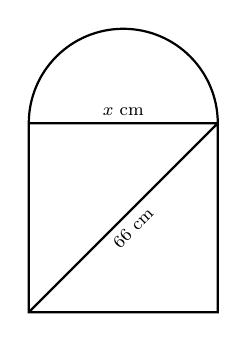
\begin{tikzpicture}[smooth,font=\footnotesize,scale=0.8,thick]
		\path
		(0,0) coordinate (O)
		(-1.5,0) coordinate (A)
		(1.5,0) coordinate (B)
		(1.5,-3) coordinate (C)
		(-1.5,-3) coordinate (D)
		;
		\draw 
		(A)--(B)--(C)--(D)--cycle
		(D)--(B)
		(0:1.5 cm) arc (0:180:1.5 cm);
		\path 
		(D)--(B) node[below,midway,sloped,scale=.8]{$66$ cm }
		(B)--(A) node[above,midway,scale=.8]{$x$ cm }
		;
	
\end{tikzpicture}}
	\loigiai{
	Gọi đường kính của nửa hình tròn là $x(\mathrm{~cm})(x>0)$. Độ dài cạnh bên của hình chữ nhật là $\sqrt{66^{2}-x^{2}}$. Diện tích nửa hình tròn là $\frac{3,14 x^{2}}{8}$. Diện tích hình chữ nhật là $x \sqrt{66^{2}-x^{2}}$. Theo giả thiết ta có:
	$$
	\begin{aligned}
		\dfrac{3,14 x^{2}}{8}=0,3 x \sqrt{66^{2}-x^{2}} & \Leftrightarrow 157 x=120 \sqrt{66^{2}-x^{2}} \\
		& \Leftrightarrow x^{2}=\dfrac{62726400}{39049} \Leftrightarrow x \approx \pm 40,08 .
	\end{aligned}
	$$
	Vậy kích thước của hình chữ nhật khoảng $40,08 \mathrm{~cm} \times 52,44 \mathrm{~cm}$.}
\end{vd}

\begin{vd}
	Một công ty muốn làm một đường ống dẫn từ một điểm $A$ trên bờ đến một điểm $C$ trên một hòn đảo. Hòn đảo cách bờ biển $6 \mathrm{~km}$. Để thực hiện, công ty dự định xây dựng phần đường ống trên bờ từ A đến B và đường ống dưới nước từ B đến C (hình vẽ). 
	\begin{center}
		\begin{tikzpicture}[scale=0.25, font=\footnotesize, line join=round, line cap=round, >=stealth]
			\def\m{1}
			\begin{scope}%[opacity=0.75]
				\clip(-30,10)rectangle(10,-10);
				\fill[cyan!20,,opacity=0.5](-30,10)rectangle(10,-10);
				\fill[orange!30!brown,opacity=0.5](-30,0)rectangle(10,-10);
				\fill [left color=brown!60!green,right color=brown!30!orange,line width=1.5pt,->,decorate,
				decoration={snake,amplitude=0.5mm,segment length=0.5 cm,post length=0.5 mm}](-10,0)..controls++(20:5) and++(-140:2)..(0,3)..controls++(-70:2) and++(170:3)..(10,0)--cycle;
				\tikzset{co/.pic={
						\fill[green!80!teal,out=110,in=-20] (0,0)to(-1,1)[out=-10,in=120]to(-0.2,0.7)[out=110,in=-20]to(0,1.5)[out=-40,in=100]to(0.5,0.5)[out=40,in=-120]to(1,1.3)--(0.75,0)--cycle;
				}}
				\foreach \x/\y [count=\i]in{-3/0.2,-5/0.7,5/0.2,3/0.4,0/1.2,-8/0,-2/2}
				\path(\x,\y)pic[xslant=\i/30,yscale=\i/5]{co};
				\fill [cyan,decorate,
				decoration={snake,amplitude=0.5mm,segment length=1 cm,post length=0.5 mm},,opacity=0.5]
				(-40,0.25)--++(80,0)--++(-90:5)..controls++(-140:10) and++(-150:5)..(-20,-5)--cycle;
				\tikzset{Icon-mattroi/.pic={
						\def\r{0.35}
						\fill(0,0)circle(\r);
						\draw[line width=2*\r pt](0,0)circle(\r);
						\foreach \g in{1,...,10}{
							\draw[line width=5 pt](\g*36:1.2*\r)++(\g*36:0.1*\r)--++(\g*36:\r*0.25);
						}
				}}
				%%Mây
				\tikzset{Icon-may/.pic={
						\def\r{0.35}
						\fill[white,line width=2.5*\r pt](-\r,0)--(\r,0)..controls++(0:\r) and ++(30:\r)..(0.8*\r,\r)..controls++(100:\r) and ++(80:\r)..(-0.75*\r,0.8*\r)..controls++(140:\r) and++(180:\r)..(-\r,0);
				}}
				%%Hết mây
				\begin{scope}
					\def\l{5}
					\tikzset{la/.pic={
							\fill[green!60!teal,out=15,in=172](0,0)to(\l,0)[out=176,in=5]to(0,0);
							\draw[green,out=10,in=174](0,0)to(\l,0);
					}}
					\begin{scope}[shift={(-25,-6.75)},yellow,scale=0.5]
						\draw[line width=3pt](0,15)..controls++(-160:5) and++(110:2)..(-5,7)foreach \i in{1,2,...,20}{coordinate[pos=\i/20](A\i)};
						\foreach \i in{1,2,...,20}
						\path(A\i)pic[rotate={-70+\i},scale=1-\i/40]{la}(A\i)pic[rotate={-90+\i},scale=1-\i/40]{la};
						%Lá 2
						\draw[line width=3pt](0,15)..controls++(160:5) and++(60:2)..(-10,12)foreach \i in{1,2,...,20}{coordinate[pos=\i/20](A\i)};
						\foreach \i in{1,2,...,20}
						\path(A\i)pic[rotate={-80+\i},scale=1-\i/40]{la}(A\i)pic[rotate={-95+\i},scale=0.9-\i/30]{la};
						%Lá 3
						\draw[line width=2pt](0,15)..controls++(110:5) and++(-10:2)..(-7,20)foreach \i in{1,2,...,20}{coordinate[pos=\i/20](A\i)};
						\foreach \i in{1,2,...,20}
						\path(A\i)pic[rotate={-170+\i},scale=1-\i/40,,xscale=0.75]{la}(A\i)pic[rotate={80+\i},scale=1-\i/40,xscale=0.75]{la};
						%Lá 4
						\draw[line width=2pt](0,15)..controls++(70:5) and++(-170:2)..(7,20)foreach \i in{1,2,...,20}{coordinate[pos=\i/20](A\i)};
						\foreach \i in{1,2,...,20}
						\path(A\i)pic[rotate={50+\i},scale=1-\i/40,,xscale=0.75]{la}(A\i)pic[rotate={-20+\i},scale=1-\i/40,xscale=0.75]{la};
						%Lá 5
						\draw[line width=2pt](0,15)..controls++(20:5) and++(100:2)..(5,7)foreach \i in{1,2,...,20}{coordinate[pos=\i/20](A\i)};
						\foreach \i in{1,2,...,20}
						\path(A\i)pic[rotate={-90+\i},scale=1-\i/40,,xscale=0.75]{la}(A\i)pic[rotate={-50+\i},scale=1-\i/40,xscale=0.75]{la};
						%Lá 6
						\draw[line width=2pt](0,15)..controls++(90:5) and++(-130:2)..(2,22)foreach \i in{1,2,...,20}{coordinate[pos=\i/20](A\i)};
						\foreach \i in{1,2,...,20}
						\path(A\i)pic[rotate={110+\i},scale=1-\i/40,,xscale=0.75]{la}(A\i)pic[rotate={50+\i},scale=1-\i/40,xscale=0.75]{la};
					\end{scope}
					\tikzset{qua/.pic={
							\fill[green, draw=teal](1,0)arc(0:360:0.8 and 1);
					}}
					%%Thân 
					\tikzset{than/.pic={
							\fill[brown!40!black,line width=2pt](-3,0)..controls++(30:4) and++(-70:2)..(-0.5,15)foreach \i in{1,2,...,20}{coordinate[pos=\i/20](A\i)}--(0.5,15)..controls++(-70:4) and++(70:2)..(0.5,0)foreach \i in{1,2,...,20}{coordinate[pos=\i/20](B\i)}--cycle;}}
					%%Gôc
					\tikzset{da/.pic={
							\fill[ball color=gray!40!brown](0,0)..controls++(50:2) and++(160:1)..(4,0)..controls++(40:5) and++(130:3)..(10,0)..controls++(-110:2) and++(-140:3)..(0,0);
					}}
					\path(-25,-8)pic[scale=0.5]{than}(-28,-8)pic[scale=0.75]{da}(-24,0.5)pic[scale=0.75]{qua}(-26,0.5)pic[scale=0.75]{qua}(-25,0.25)pic[scale=0.75]{qua};
				\end{scope}
				\draw[line width=3pt,orange](6,0.5)coordinate(C)--++(-120:10)coordinate(B)--++(180:15)coordinate(A)($(A)!(C)!(B)$)coordinate(H);
				\draw[dashed](C)--(H)node[pos=0.5,right]{$6$ km}--(B);
			\end{scope}
			\foreach \d/\g in{C/90,H/0,B/110,A/180}
			\draw[fill=black](\d)circle(1pt)node[shift={(\g:0.5)}]{$\d$};
			\draw[<->,dashed]([shift={(0,-1)}]A)--([shift={(0,-1)}]H)node[below,pos=0.6]{$9$ km};
		\end{tikzpicture}
	\end{center}
	 Biết giá để xây đường ống trên bờ là $50.000 \mathrm{USD}$ mỗi km, và $130.000 \mathrm{USD}$ mỗi km để xây dưới nước. Xác định đoạn đường từ $A$ đến $B$ để tổng chi phí xây dựng lăp đặt từ A đến C khoảng 1.170.000 USD.
	 \loigiai{
	 Đặt $x=BH$, $x \in[0 ; 9]$. Khi đó
	 $$
	 BC=\sqrt{x^2+36};\, AB=9-x
	 $$
	 Chi phí xây dựng đường ống là
	 $$
	 C(x)=130.000 \sqrt{x^{2}+36}+50.000(9-x)
	 $$
	 Để chi phí khoảng 1.170.000, ta có phương trình
	 $$130.000 \sqrt{x^{2}+36}+50.000(9-x)=1.170.000 \Leftrightarrow x=\dfrac{5}{2}$$
	 Suy ra $AB=9-x=6,5$ km.}
\end{vd}
\subsection{BÀI TẬP TỰ LUYỆN}

\begin{bt}%[0D4B5-6]
	Giải các phương trình sau:
	\begin{listEX}[2]
		\item $\sqrt{2x^2-3x-1}=\sqrt{2x+3}$.
		\item $\sqrt{4x^2-6x-6}=\sqrt{x^2-6}$.
		\item $\sqrt{x+9}=2x-3$.
		\item $\sqrt{-x^2+4x-2}=2-x$.
		\item $\sqrt{2-x}+2x=3$
		\item $\sqrt{-x^2+7x-6}+x=4$
	\end{listEX}
	\loigiai{
		\begin{listEX}[1]
			\item \begin{eqnarray*}
				&&\sqrt{2x^2-3x-1}=\sqrt{2x+3}\\
				&\Leftrightarrow& \heva{&2x+3\ge 0\\&2x^2-3x-1=2x+3}\\
				&\Leftrightarrow& \heva{&x\ge \dfrac{-3}{2}\\&2x^2-5x-4=0}\\
				&\Leftrightarrow& \heva{&x\ge \dfrac{-3}{2}\\&x=\dfrac{5\pm\sqrt{57}}{4}}\\
				&\Leftrightarrow& x=\dfrac{5\pm\sqrt{57}}{4}.
			\end{eqnarray*}	
			Vậy tập nghiệm là $S=\left\{\dfrac{5-\sqrt{57}}{4};\dfrac{5+\sqrt{57}}{4}\right\}$.	
			\item
			\begin{eqnarray*}
				&&\sqrt{4x^2-6x-6}=\sqrt{x^2-6}\\
				&\Leftrightarrow& \heva{&x^2-6\ge 0\\&4x^2-6x-6=x^2-6}\\
				&\Leftrightarrow& \heva{&x^2-6\ge 0\\&3x^2-6x=0}\\
				&\Leftrightarrow& \heva{&\hoac{&x\le -\sqrt{6}\\&x\ge \sqrt{6}}\\&\hoac{&x=0\\&x=2}}\\
				&\Leftrightarrow& x\in \varnothing .
			\end{eqnarray*}
			Vậy phương trình vô nghiệm.
			\item 
			\begin{eqnarray*}
				&&\sqrt{x+9}=2x-3\\
				&\Leftrightarrow& \heva{&2x-3\ge 0\\&x+9=4x^2-12x+9}\\
				&\Leftrightarrow& \heva{&x\ge \dfrac{3}{2}\\&4x^2-13x=0}\\
				&\Leftrightarrow& \heva{&x\ge \dfrac{3}{2}\\&\hoac{&x=0\\&x=\dfrac{13}{4}}}\\
				&\Leftrightarrow& x=\dfrac{13}{4}.
			\end{eqnarray*}	
			Vậy tập nghiệm là $S=\left\{\dfrac{13}{4}\right\}$.	
			\item
			\begin{eqnarray*}
				&&\sqrt{-x^2+4x-2}=2-x\\
				&\Leftrightarrow& \heva{&2-x\ge 0\\&-x^2+4x-2=x^2-4x+4}\\
				&\Leftrightarrow& \heva{&x\le 2\\&2x^2-8x+6=0}\\
				&\Leftrightarrow& \heva{&x\le 2\\&\hoac{&x=1\\&x=3}}\\
				&\Leftrightarrow& x=1.
			\end{eqnarray*}	
			Vậy tập nghiệm là $S=\{1\}$.	
			\item 
			\begin{eqnarray*}
				&&\sqrt{2-x}+2x=3\\
				&\Leftrightarrow&\sqrt{2-x}=3-2x\\
				&\Leftrightarrow& \heva{&3-2x\ge 0\\&2-x=4x^2-12x+9}\\
				&\Leftrightarrow& \heva{&x\le \dfrac{3}{2}\\&4x^2-11x+7=0}\\
				&\Leftrightarrow& \heva{&x\le \dfrac{3}{2}\\&\hoac{&x=1\\&x=\dfrac{7}{4}}}\\
				&\Leftrightarrow& x=1.
			\end{eqnarray*}	
			Vậy tập nghiệm là $S=\{1\}$.	
			\item 
			\begin{eqnarray*}
				&&\sqrt{-x^2+7x-6}+x=4\\
				&\Leftrightarrow&\sqrt{-x^2+7x-6}=4-x\\
				&\Leftrightarrow& \heva{&4-x\ge 0\\&-x^2+7x-6=x^2-8x+16}\\
				&\Leftrightarrow& \heva{&x\le 4\\&2x^2-15x+22=0}\\
				&\Leftrightarrow& \heva{&x\le 4\\&\hoac{&x=2\\&x=\dfrac{11}{2}}}\\
				&\Leftrightarrow& x=\dfrac{13}{4}.
			\end{eqnarray*}	
			Vậy tập nghiệm là $S=\{2\}$.	
		\end{listEX}
	} 
\end{bt}




\begin{bt}
	\immini{Cho tam giác $ABC$ và $ABD$ cùng vuông tại $A$ như hình bên với $AB=x$, $BC=5$ và $BD=6$.
	\begin{enumEX}[a)]{1}
		\item Biểu diễn độ dài cạnh $AC$ và $AD$ theo $x$.
		\item Tìm $x$ đề chu vi của tam giác $ABC$ là $12$ .
		\item Tìm $x$ để $AD=2AC$.
	\end{enumEX}}{
	\begin{tikzpicture}[smooth,scale=1.2]
		\path
		(0,0) coordinate (A)
		(-2.7,0) coordinate (D)
		(2,0) coordinate (C)
		(0,1.5) coordinate (B)
		;
		\draw (B)--(C)--(D)--cycle (A)--(B)
		pic[draw, angle radius=2mm]{right angle=C--A--B}
		;
		\path 
		(A)--(B) node[right,midway,scale=.8]{$x$ }
		(D)--(B) node[above,midway,sloped,scale=.8]{$6$ }
		(C)--(B) node[above,midway,sloped,scale=.8]{$5$ }
		;
		\foreach \x/\g in {A/-90,D/-90,C/-90,B/90} \draw[fill=black] (\x) circle (.05) +(\g:.3) node{$\x$};
\end{tikzpicture}}
\loigiai{
	\begin{enumerate}[a)]
		\item Vì $x$ là khoảng cách $AN$ nên $x \geq 0$.
		$$
		\begin{aligned}
			AC=\sqrt{AN^2+NC^2-2 AN \cdot NC \cdot \cos 60^{\circ}} &=\sqrt{x^2+100-10x} \\
			BC=\sqrt{BN^2+NC^2-2 BN \cdot NC \cdot \cos 60^{\circ}} &=\sqrt{(x+3)^{2}+100-10(x+3)} \\
			&=\sqrt{x^{2}-4 x+79} .
		\end{aligned}
		$$
		\item Ta có $AC=\dfrac{8}{9} BC$
		$$
		\begin{aligned}
			&\Rightarrow \sqrt{x^{2}-10 x+100}=\dfrac{8}{9} \sqrt{x^{2}-4 x+79} \\
			&\Rightarrow 81\left(x^{2}-10 x+100\right)=64\left(x^{2}-4 x+79\right) \\
			&\Rightarrow 17 x^{2}-554 x+3044=0 \\
			&\Rightarrow x \approx 25,6 \text { hoặc } x \approx 7 .
		\end{aligned}
		$$
		Vậy $x \approx 25,6$ hoặc $x \approx 7$.
		\item Ta có $BC=2 AN$
		$$
		\begin{aligned}
			&\Rightarrow \sqrt{x^{2}-4 x+79}=2 x \\
			&\Rightarrow x^{2}-4 x+79=4 x^{2} \\
			&\Rightarrow 3 x^{2}+4 x-79=0 \\
			&\Rightarrow x \approx 4,5 \text { hoặc } x \approx-5,8 .
		\end{aligned}
		$$
		Mà vì $x \geq 0$ nên ta có $x \approx 4,5$.
\end{enumerate}}
\end{bt}
\begin{bt}%[0D3B3-5]
	Một kĩ sư thiết kế đường dây điện từ vị trí $A$ đến vị trí $S$ và từ vị trí $S$ đến vị trí $C$ trên cù lao như hình bên. 	\begin{center}
		\begin{tikzpicture}[scale=0.3, font=\footnotesize, line join=round, line cap=round, >=stealth]
			\def\m{1}
			\begin{scope}%[opacity=0.75]
				\clip(-30,10)rectangle(10,-10);
				\fill[cyan!20,,opacity=0.5](-30,10)rectangle(10,-10);
				\fill[orange!30!brown,opacity=0.5](-30,0)rectangle(10,-10);
				\fill [left color=brown!60!green,right color=brown!30!orange,line width=1.5pt,->,decorate,
				decoration={snake,amplitude=0.5mm,segment length=0.5 cm,post length=0.5 mm}](-10,0)..controls++(20:5) and++(-140:2)..(0,3)..controls++(-70:2) and++(170:3)..(10,0)--cycle;
				\tikzset{co/.pic={
						\fill[green!80!teal,out=110,in=-20] (0,0)to(-1,1)[out=-10,in=120]to(-0.2,0.7)[out=110,in=-20]to(0,1.5)[out=-40,in=100]to(0.5,0.5)[out=40,in=-120]to(1,1.3)--(0.75,0)--cycle;
				}}
				\foreach \x/\y [count=\i]in{-3/0.2,-5/0.7,5/0.2,3/0.4,0/1.2,-8/0,-2/2}
				\path(\x,\y)pic[xslant=\i/30,yscale=\i/5]{co};
				\fill [cyan,decorate,
				decoration={snake,amplitude=0.5mm,segment length=1 cm,post length=0.5 mm},,opacity=0.5]
				(-40,0.25)--++(80,0)--++(-90:5)..controls++(-140:10) and++(-150:5)..(-20,-5)--cycle;
				\tikzset{Icon-mattroi/.pic={
						\def\r{0.35}
						\fill(0,0)circle(\r);
						\draw[line width=2*\r pt](0,0)circle(\r);
						\foreach \g in{1,...,10}{
							\draw[line width=5 pt](\g*36:1.2*\r)++(\g*36:0.1*\r)--++(\g*36:\r*0.25);
						}
				}}
				%%Mây
				\tikzset{Icon-may/.pic={
						\def\r{0.35}
						\fill[white,line width=2.5*\r pt](-\r,0)--(\r,0)..controls++(0:\r) and ++(30:\r)..(0.8*\r,\r)..controls++(100:\r) and ++(80:\r)..(-0.75*\r,0.8*\r)..controls++(140:\r) and++(180:\r)..(-\r,0);
				}}
				%%Hết mây
					\begin{scope}
					\def\l{5}
					\tikzset{la/.pic={
							\fill[green!60!teal,out=15,in=172](0,0)to(\l,0)[out=176,in=5]to(0,0);
							\draw[green,out=10,in=174](0,0)to(\l,0);
					}}
					\begin{scope}[shift={(-25,-6.75)},yellow,scale=0.5]
						\draw[line width=3pt](0,15)..controls++(-160:5) and++(110:2)..(-5,7)foreach \i in{1,2,...,20}{coordinate[pos=\i/20](A\i)};
						\foreach \i in{1,2,...,20}
						\path(A\i)pic[rotate={-70+\i},scale=1-\i/40]{la}(A\i)pic[rotate={-90+\i},scale=1-\i/40]{la};
						%Lá 2
						\draw[line width=3pt](0,15)..controls++(160:5) and++(60:2)..(-10,12)foreach \i in{1,2,...,20}{coordinate[pos=\i/20](A\i)};
						\foreach \i in{1,2,...,20}
						\path(A\i)pic[rotate={-80+\i},scale=1-\i/40]{la}(A\i)pic[rotate={-95+\i},scale=0.9-\i/30]{la};
						%Lá 3
						\draw[line width=2pt](0,15)..controls++(110:5) and++(-10:2)..(-7,20)foreach \i in{1,2,...,20}{coordinate[pos=\i/20](A\i)};
						\foreach \i in{1,2,...,20}
						\path(A\i)pic[rotate={-170+\i},scale=1-\i/40,,xscale=0.75]{la}(A\i)pic[rotate={80+\i},scale=1-\i/40,xscale=0.75]{la};
						%Lá 4
						\draw[line width=2pt](0,15)..controls++(70:5) and++(-170:2)..(7,20)foreach \i in{1,2,...,20}{coordinate[pos=\i/20](A\i)};
						\foreach \i in{1,2,...,20}
						\path(A\i)pic[rotate={50+\i},scale=1-\i/40,,xscale=0.75]{la}(A\i)pic[rotate={-20+\i},scale=1-\i/40,xscale=0.75]{la};
						%Lá 5
						\draw[line width=2pt](0,15)..controls++(20:5) and++(100:2)..(5,7)foreach \i in{1,2,...,20}{coordinate[pos=\i/20](A\i)};
						\foreach \i in{1,2,...,20}
						\path(A\i)pic[rotate={-90+\i},scale=1-\i/40,,xscale=0.75]{la}(A\i)pic[rotate={-50+\i},scale=1-\i/40,xscale=0.75]{la};
						%Lá 6
						\draw[line width=2pt](0,15)..controls++(90:5) and++(-130:2)..(2,22)foreach \i in{1,2,...,20}{coordinate[pos=\i/20](A\i)};
						\foreach \i in{1,2,...,20}
						\path(A\i)pic[rotate={110+\i},scale=1-\i/40,,xscale=0.75]{la}(A\i)pic[rotate={50+\i},scale=1-\i/40,xscale=0.75]{la};
					\end{scope}
					\tikzset{qua/.pic={
							\fill[green, draw=teal](1,0)arc(0:360:0.8 and 1);
					}}
					%%Thân 
					\tikzset{than/.pic={
							\fill[brown!40!black,line width=2pt](-3,0)..controls++(30:4) and++(-70:2)..(-0.5,15)foreach \i in{1,2,...,20}{coordinate[pos=\i/20](A\i)}--(0.5,15)..controls++(-70:4) and++(70:2)..(0.5,0)foreach \i in{1,2,...,20}{coordinate[pos=\i/20](B\i)}--cycle;}}
					%%Gôc
					\tikzset{da/.pic={
							\fill[ball color=gray!40!brown](0,0)..controls++(50:2) and++(160:1)..(4,0)..controls++(40:5) and++(130:3)..(10,0)..controls++(-110:2) and++(-140:3)..(0,0);
					}}
					\path(-25,-8)pic[scale=0.5]{than}(-28,-8)pic[scale=0.75]{da}(-24,0.5)pic[scale=0.75]{qua}(-26,0.5)pic[scale=0.75]{qua}(-25,0.25)pic[scale=0.75]{qua};
				\end{scope}
			
				\draw(6,0.5)coordinate(C)--++(-120:10)coordinate(S)--++(180:15)coordinate(A)($(A)!(C)!(S)$)coordinate(B);
				\draw[dashed](C)--(B)node[pos=0.5,right]{$1$ km}--(S);
			\end{scope}
			\foreach \d/\g in{C/90,B/0,S/110,A/180}
			\draw[fill=black](\d)circle(1pt)node[shift={(\g:0.5)}]{$\d$};
			\draw[<->,dashed]([shift={(0,-1)}]A)--([shift={(0,-1)}]B)node[below,pos=0.6]{$4$ km};
		\end{tikzpicture}
	\end{center}
Tiền công thiết kế mỗi ki-lô-mét đường dây từ $A$ đến $S$ và từ $S$ đến $C$ lần lượt là $3$ triệu đồng và $5$ triệu đồng. Biết tổng số tiền công là $16$ triệu đồng. Tính tổng số ki-lô-mét đường dây đã thiết kế. 
	\loigiai{
		Đặt $BS=x$ (ki-lô-mét) với $0<x<4$. Suy ra $AS=4-x$.\\
		Áp dụng định lý Pi-ta-go trong tam giác $BCS$ ta có $CS=\sqrt{1+x^2}$ (ki-lô-mét).\\
		Tổng số tiền để lắp đặt là $5\sqrt{1+x^2}+3(4-x)$ (triệu đồng).\\
		Vì tổng chi phí lắp đặt là $16$ triệu đồng, nên ta có phương trình
		\begin{eqnarray*}
			&& 5\sqrt{1+x^2}+3(4-x)=16\Leftrightarrow 5\sqrt{1+x^2}=4+3x \\
			&\Leftrightarrow & 25(1+x^2)=16+24x+9x^2 \,\,(x>0)\\
			&\Leftrightarrow & 16x^2-24x+9=0\Leftrightarrow x=\dfrac{3}{4}\,\,(\text{thỏa điều kiện }\,\,0<x<4).
		\end{eqnarray*}
		Tổng quãng đường đã thiết kế là 
		\[\ell=\sqrt{1+\dfrac{9}{16}}+4-\dfrac{3}{4}=\dfrac{9}{2}\,\,(\text{ki-lô-mét}).\]
	}
\end{bt}

\begin{bt}
	Để leo lên một bức tường, bác Nam dùng một chiếc thang có chiều dài cao hơn bức tường đó $1$ m. Ban đầu, bác Nam đặt chiếc thang mà đầu trên của chiếc thang đó vừa chạm đúng vào mép trên bức tường (Hình $33 a$). Sau đó, bác Nam dịch chuyển chân thang vào gần chân tường thêm $0,5$ m thì bác Nam nhận thấy thang tạo với mặt đất một góc $60^{\circ}$ (Hình 33b). Bức tường cao bao nhiêu mét (làm tròn kết quả đến hàng phần mười)?
	\begin{center}
		\begin{tikzpicture}[scale=0.6, font=\footnotesize, line join=round, line cap=round, >=stealth]
			\begin{scope}[font=\footnotesize, >=stealth]
				\draw[line width=0.1cm,shift={(2,-1)}] (-2,4.3)coordinate (E)--(6,0)coordinate (F);
				\path 
				(2.5,-1.1) coordinate (B) node [below]{$B$}
				(5.5,6.85) coordinate (A)node [above]{$A$}
				($(E)!{2/3}!(F)$) coordinate (C)node [below]{$C$}
				($(A)-(C)$) coordinate (T)
				($(T)+(2,-1)$) coordinate (R)
				($(T)+(2,0)$) coordinate (W)
				;
				\draw[line width=0.1cm,shift={(R)}] (-2,4.3)--(6,0);
				\draw[line width=0.1cm,shift={(W)}] (-2,4.3)--(6,0);
				\draw pic[draw,line width=0.1cm,angle radius=8]{right angle=A--C--B};	
				\draw[line width=0.7cm,teal] (0,0)--(3,8);
				\draw[line width=0.7cm,teal,shift={(2,-1)}] (0,0)--(3,8);
				\foreach \x in {1,2,...,7}{
					\pgfmathsetmacro{\a}{(3*\x/8)}
					\pgfmathsetmacro{\b}{(8*\x/8)}
					\draw[line width=0.3cm,teal,shift={(\a,\b)}] (0,0)--(2,-1);
				}
				\draw[line width=0.1cm,line join=round, line cap=round,] (A)--(C)--(B)--cycle;	
				\path 
				(3,-2) coordinate (TT) node [below]{$a)$};
			\end{scope}
			\begin{scope}[font=\footnotesize, >=stealth,xshift=10cm]
				\draw[line width=0.1cm,shift={(2,-1)}] (-2,4.3)coordinate (H)--(6,0)coordinate (K);
				\path 
				(2.5,-1.05) coordinate (E) node [below]{$E$}
				(4.25,6.6) coordinate (D)node [above right]{$D$}
				($(H)!{1/2}!(K)$) coordinate (G)node [above right]{$G$}
				($(D)-(G)$) coordinate (T)
				($(T)+(2,-1)$) coordinate (R)
				($(T)+(2,0)$) coordinate (W)
				;
				\draw[line width=0.1cm,shift={(R)}] (-2,4.3)--(6,0);
				\draw[line width=0.1cm,shift={(W)}] (-2,4.3)--(6,0);
				\draw pic[draw,line width=0.1cm,angle radius=10]{right angle=D--G--E};
				\draw pic[draw,angle radius=20]{angle=G--E--D}(E)node[shift={(63:1.3)}]{$60^\circ$};
				\draw[line width=0.7cm,teal] (0,0)--(2,9);
				\draw[line width=0.7cm,teal,shift={(2,-1)}] (0,0)--(2,9);	
				\foreach \x in {1,2,...,7}{
					\pgfmathsetmacro{\a}{(2*\x/8)}
					\pgfmathsetmacro{\b}{(9*\x/8)}
					\draw[line width=0.3cm,teal,shift={(\a,\b)}] (0,0)--(2,-1);
				}
				\draw[line width=0.1cm,line join=round, line cap=round,] (D)--(G)--(E)--cycle;
				\path 
				(3,-2) coordinate (TTT) node [below]{$b)$};		
			\end{scope}
			\path 
			(8,-3) coordinate (TTTT) node [below]{Hình 33};	
		\end{tikzpicture}
	\end{center}
	
	\loigiai{
		Theo giả thiết ta có $AB=AC+1$, $DG=AC$ và $EG=CB-0{,}5$ với ($AB>1,BC>0{,}5$).\\
		Tam giác $DGE$ vuông tại $G$ nên: $\tan 60^{\circ}=\dfrac{DG}{GE}=\dfrac{AC}{BC-0{,}5}\Rightarrow AC=\sqrt{3}\cdot(BC-0{,}5)$.\\
		Tam giác $ABC$ vuông tại $C$ nên ta có:
		\begin{eqnarray*}
			AB^2=BC^2+AC^2&\Leftrightarrow& (AC+1)^2=BC^2+AC^2\\
			&\Leftrightarrow& BC^2=2AC+1\\
			&\Leftrightarrow& BC^2-2\sqrt{3}BC+\sqrt{3}-1=0\\
			&\Leftrightarrow&\heva{&BC=\sqrt{3}-\sqrt{4-\sqrt{3}}\approx 0{,}2 \quad \textrm{(loại)}\\&BC=\sqrt{3}+\sqrt{4-\sqrt{3}}\approx 3{,}2.}
		\end{eqnarray*}
		Với $BC=\sqrt{3}+\sqrt{4-\sqrt{3}}$ ta có $AC=\sqrt{3}\left(\sqrt{3}+\sqrt{4-\sqrt{3}}-0{,}5\right)\approx 4{,}7$.\\
		Vậy chiều cao bức tường là $AC\approx 4{,}7$ m.
	} 
\end{bt}

\begin{bt}%[0D4B5-6]
	\immini
	{Một người đứng ở điểm $A$ trên một bờ sông rộng $300$ m, chèo thuyền đến vị trí $D$, sau đó chạy bộ đến vị trí $B$ cách C một khoảng $800$ m như Hình 34. Vận tốc chèo thuyền là $6$ km/h, vận tốc chạy bộ là $10$ km/h và giả sử vận tốc dòng nưốc không đáng kể. Tính khoảng cách từ vị trí $C$ đến $D$, biết tổng thời gian người đó chèo thuyền và chạy bộ từ $A$ đến $B$ là $7{,}2$ phút.}
	{
		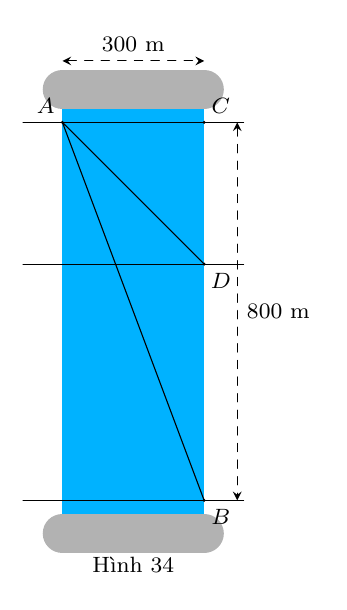
\begin{tikzpicture}[scale=0.6, font=\footnotesize, line join=round, line cap=round, >=stealth]
			\fill[blue!30!cyan] (0,-8.5) rectangle (3,0.5);
			\path 
			(0,0) coordinate (A)
			(3,0) coordinate (C)
			(3,-3) coordinate (D)
			(3,-8) coordinate (B)
			(1.5,-9) coordinate (FF) node[below]{Hình 34}
			;
			\foreach  \x in {0,-3,-8}{
				\draw[shorten <= -0.5cm,shorten >= -0.5cm,shift={(0,\x)}] (0,0)--(3,0);
			}	
			\foreach  \x in {0.7,-8.7}{
				\draw[shift={(0,\x)},line width=0.5cm,black!30] (0,0)--(3,0);
			}	
			\draw[<->,dashed] (0,1.3)--(3,1.3) node[above,midway]{$300$ m};
			\draw (B)--(A)--(D);
			\draw[<->,dashed] (3.7,0)--(3.7,-8) node[right,midway]{$800$ m};
			\foreach \p/\g in {A/135,B/-45,C/45,D/-45}\fill[black] (\p) circle (1pt) +(\g:.5)node{$\p$};
	\end{tikzpicture}}
	\loigiai{
		Gọi $CD=a$ km suy ra $BD=0{,}8-a$ km ($0<a< 0{,}8$).\\
		Theo giả thiết ta có $AD=\sqrt{AC^2+CD^2}=\sqrt{0{,}3^2+a^2}$.\\
		Từ đó suy ra \begin{eqnarray*}
			&&\dfrac{\sqrt{0{,}3^2+a^2}}{6}+\dfrac{0{,}8-a}{10}=\dfrac{7{,}2}{60}\\
			&\Leftrightarrow & \sqrt{0{,}09+a^2}=0{,}6a+0{,}24\\
			&\Leftrightarrow & 0{,}09+a^2=0{,}36a^2+0{,}288a+0{,}0576\\
			&\Leftrightarrow & 0{,}64a^2-0{,}288a+0{,}0324=0\\
			&\Leftrightarrow & a=0{,}225.
		\end{eqnarray*}
		Vậy $CD=0{,}225$ km $=225$ m.	
	} 
\end{bt}

\begin{bt}%[0D4B5-6]
	\immini
	{Một ngọn hải đăng đặt tại vị trí $A$ cách bờ biển một khoảng cách $A B=4$ km. Trên bờ biển có một cái kho ở vị trí $C$ cách $B$ một khoảng là $7$ km. Người canh hải đăng có thể chèo thuyền từ $A$ đến vị trí $M$ trên bờ biển vối vận tốc $3$ km/h rồi đi bộ đến $C$ với vận tốc $5$ km/h như Hình 35 . Tính khoảng cách từ vị trí $B$ đến $M$, biết thời gian người đó đi từ $A$ đến $C$ là 148 phút.}
	{\begin{tikzpicture}[scale=0.7, font=\footnotesize, line join=round, line cap=round, >=stealth]
			\path 
			(0,4) coordinate (A)
			(0,0) coordinate (B)
			(7,0) coordinate (C)
			(3,0) coordinate (M)
			(3.5,-1) coordinate (TT) node [below]{Hình 35}
			;
			\draw (B)--(A)node[left,midway]{$4$ km}--(M);
			\draw[shorten <= -0.5cm,shorten >= -0.5cm] (B)--(C);
			\draw[dashed] (B)--+(0,-0.5)(C)--+(0,-0.5);
			\draw[<->,dashed,yshift=-0.3cm] (0,0)--(7,0) node[below,midway]{$7$ km};
			\foreach \p/\g in {A/90,B/135,C/90,M/45}\fill[black] (\p) circle (1pt) +(\g:.5)node{$\p$};
	\end{tikzpicture}}
	\loigiai{
		Gọi $BM=a$ km suy ra $MC=7-a$ km ($0<a<7$).\\
		Theo giả thiết ta có $AM=\sqrt{AB^2+BM^2}=\sqrt{4^2+a^2}$.\\
		Từ đó suy ra \begin{eqnarray*}
			&&\dfrac{\sqrt{4^2+a^2}}{3}+\dfrac{7-a}{5}=\dfrac{148}{60}=\dfrac{37}{15}\\
			&\Leftrightarrow & 5\sqrt{4^2+a^2}=3a+16\\
			&\Leftrightarrow & 25(16+a^2)=9a^2+96a+256\\
			&\Leftrightarrow & 16a^2-96a+144=0\\
			&\Leftrightarrow & a=3.
		\end{eqnarray*}
		Vậy $BM=3$ km.	
	} 
\end{bt}